\section{Постановка задач}
Найти ES молекулы трифторметанол методом B3LYP/6-31G. Предположить вид TS данной молекулы. Провести оптимизацию TS методом B3LYP/6-31G и привести следующие результаты:
\begin{itemize}
    \item[-] энергия ES, TS и вклады в них;
    \item[-] высота потенциального барьера
    \item[-] определить, может ли этот барьер преодолеваться термически при комнатной температуре
\end{itemize}

\begin{figure}[H]
\centering
\captionsetup{justification=centering}
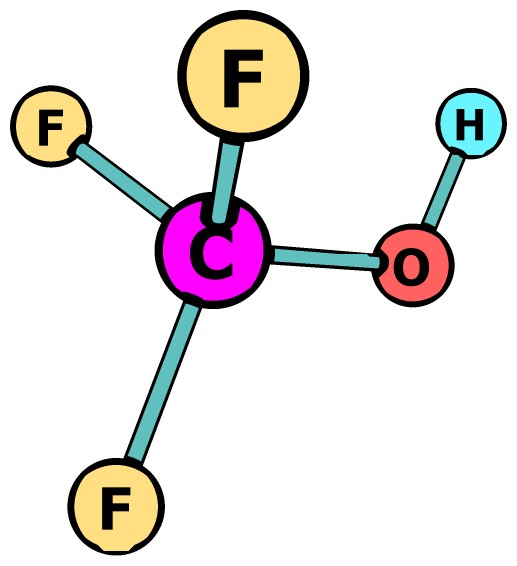
\includegraphics[scale=0.4]{fig/0.jpg}
\caption{Молекулы трифторметанол}
\end{figure}